\documentclass[12pt]{ociamthesis}  % default square logo 
%\documentclass[12pt,beltcrest]{ociamthesis} % use old belt crest logo
%\documentclass[12pt,shieldcrest]{ociamthesis} % use older shield crest logo

%load any additional packages
\usepackage{amssymb}

%input macros (i.e. write your own macros file called mymacros.tex 
%and uncomment the next line)
%\include{mymacros}

\title{Codimension-Two\\[1ex]     %your thesis title,
        Free Boundary Problems}   %note \\[1ex] is a line break in the title

\author{Keith Gillow}             %your name
\college{St Catherine's College}  %your college

%\renewcommand{\submittedtext}{change the default text here if needed}
\degree{Doctor of Philosophy}     %the degree
\degreedate{Trinity 1998}         %the degree date

%end the preamble and start the document
\begin{document}

%this baselineskip gives sufficient line spacing for an examiner to easily
%markup the thesis with comments
\baselineskip=18pt plus1pt

%set the number of sectioning levels that get number and appear in the contents
\setcounter{secnumdepth}{3}
\setcounter{tocdepth}{3}


\maketitle                  % create a title page from the preamble info
\include{dedication}        % include a dedication.tex file
\include{acknowlegements}   % include an acknowledgements.tex file
\include{abstract}          % include the abstract

\begin{romanpages}          % start roman page numbering
\tableofcontents            % generate and include a table of contents
\listoffigures              % generate and include a list of figures
\end{romanpages}            % end roman page numbering

%now include the files of latex for each of the chapters etc
\chapter{Introduksjon}
\paragraph{}I kapittel 1 ønsker gruppen å ta for seg en introduksjon av prosjektet. Dette er innledningen til selve oppgaven, og her beskrives hvem prosjektgruppen er, hvem oppdragsgiveren er, hva oppdraget er, hvilke forutsetninger og rammer prosjektet har og til slutt om strukturen på rapporten. Dette er et viktig kapittel for å få med seg informasjon om bedriften og prosjektgruppen og hvorfor prosjektet ble startet.
\section{Prosjektgruppen}
\paragraph{} Prosjektgruppen består av 4 medlemmer med ulik kompetanse og interesser. Den utgjør; Thomas Ellingsen, Erhan Sanlioglu, Mostafa Aziz og Victor Garberg Minge. Gruppen fant sammen etter å ha blitt kjent med hverandre under høstsemesteret og valgte å starte dette prosjektet sammen etter å ha snakket og diskutert sammen og kommet til enighet om at dette kan være en gruppe som kan utføre et godt prosjekt.


\begin{figure}[h]
\centering

\includegraphics[width=1.5in]{Bilder/victor2.jpg}
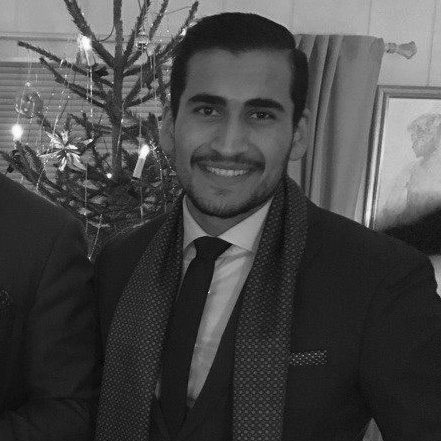
\includegraphics[width=1.5in]{Bilder/erhan2.jpg}
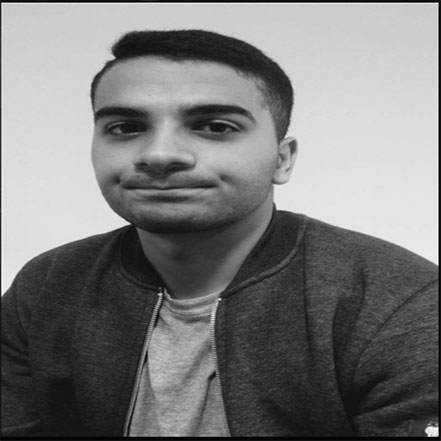
\includegraphics[width=1.5in]{Bilder/mosti2.jpg}
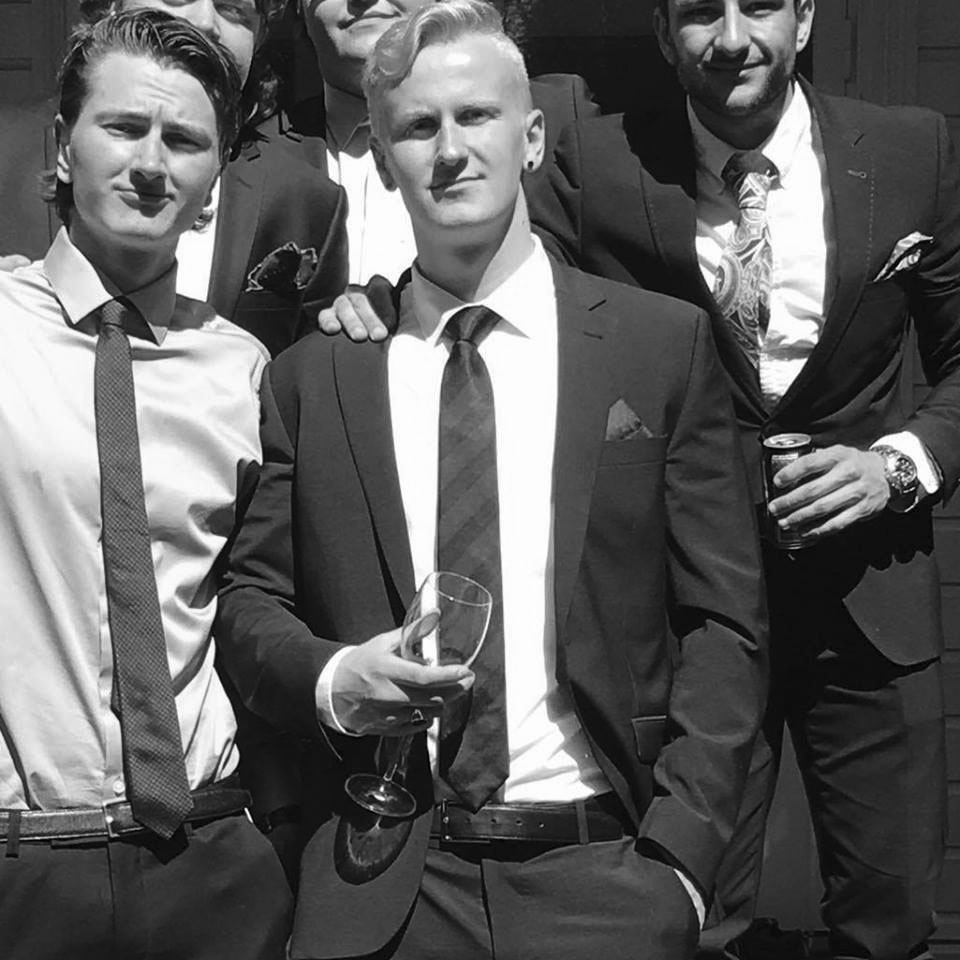
\includegraphics[width=1.5in]{Bilder/thomas2.jpg}
\end{figure}


\paragraph{} \textbf{Mostafa Aziz} er født den 01. november 1997, han valgte å studere informasjonssystemer på høgskolen i Østfold etter videregående skole. Mostafa har en rekke interesser deriblant datamaskiner og hvordan datamaskiner fungerer. Det å arbeide med servere var noe som interesserte Mostafa, ettersom det kunne være noe han kunne legge til som et område han kjenner til og ønsker å lære seg hvordan servere fungerer og hva som kan være relevant for fremtiden.




\paragraph{}\textbf{Thomas Ellingsen} født den 22.Juni 1995. Thomas har vært ett år i forsvaret og tatt utdanning som brannkostabel. I dag jobber han i Norskbrannvern hvor mesteparten av jobben går ut på kontroll og service av alarmanlegg. Thomas ønsker og kunne kombinere interessen for brann og redning med informasjonsteknologi. Derfor passet studiet informasjonssystemer på høgskolen i Østfold han perfekt. 

\paragraph{} \textbf{Victor Johannes Garberg Minge} er født den 04 August 1997. Victor studerer informasjonssystemer på Høgskolen i Østfold. Som ung har Victor alltid hatt stor interesse for det teknologiske, blandet med kreativitet falt han for linjen han nå går på Høgskolen. Victor har også en interesse for å løse problemer, noe som gjør IT et spennende område å arbeide og finne kreative løsninger. Som plan har Victor tenkt til å gjøre ferdig sin Bachelor på Høgskolen for å så se ann om videreutdanning eller arbeidslivet. Ellers har Victor en kjæreste og andre interesser deriblant idretten boksing og dataspill.

\paragraph{} \textbf{Erhan Mikael Sanlioglu} er født den 08 Desember 1994. Erhan studerer informasjonssystemer på høgskolen i Østfold. Med avlagt fagprøve og endt førstegangstjeneste kunne Erhan sette i gang med sine IT-studier på høgskolen. Erhan har hatt stor interesse for data i en tidlig alder og bestemte seg ganske tidlig for å ta en utdanning i dette feltet. Som fagarbeider har Erhan både arbeidserfaring fra det offentlige sektor og kunnskapen som trengs i dette fagfeltet. En kombinasjon som fagarbeider og en mastergrad i IT vil sikre fremtiden hans.

\section{Oppdragsgiver}

\begin{figure}[H]
\centering

\includegraphics[width=3.5in]{Bilder/katoplast_logo.png}
\caption{Katoplast logo}
\end{figure}


\paragraph{} Oppdragsgiver for prosjektet er daglig leder ved Katoplast AS, Trond Vidar Kjellin som har tillat en gruppe med studenter fra Høgskolen i Østfold å utføre et prosjekt i bedriften Katoplast AS.

\paragraph{} Bedriften ble grunnlagt i 1972 av Gunnar og Ivar kjellin. Bedriften driver produksjon, utforming, konstruksjon og materialvalg av plastprodukter. Plastproduksjonen skjer gjennom 3D-printing og gjennom støping av former. Katoplast har om lag 15-20 ansatte og selve produksjonen blir driftet av 14 forskjellige maskiner. \footnote{http://www.katoplast.no/produkter/}.

\paragraph{}Virksomheten har med årene flyttet flere ganger. I 1983 ble beslutningen tatt om å bygge egne lokaler i Tistedal, og disse var innflytningsklare på høsten 1984. Etter dette har det vært behov for flere utbygginger.\footnote{http://www.katoplast.no/om-katoplast/}.

\section{Oppdraget}
\paragraph{} Som oppdrag har prosjektgruppen blitt utdelt en rekke problemstillinger som gruppen skulle ha som utgangspunkt. Disse problemstillingene inkluderte alt fra å løse små, administrative oppgaver, til å finne store løsninger knyttet til ERP-system. Disse oppgavene inkluderte blant annet oppdatering av serverne, mye manuelt arbeid når det gjelder å legge inn data om kjøp og salg som har blitt gjort og annen informasjon om produkter og kunder.  I midlertid, valgte gruppen å gå for å løse serverproblemet som preger bedriften i stor grad. Oppdraget vil ta for seg flere, forskjellige sider ved ulike serverløsninger som kan være aktuelle for bedriften Katoplast AS

\paragraph{} I løpet av året 2016 har Katoplast opplevd problemer med sine servere, og hvordan deres IT-systemer generelt fungerer. Bedriften presenterte en rekke problemstillinger for gruppen som var IT-relaterte, og som gjorde at arbeidet deres i bedriften ikke ble gjort effektivt nok. Mye av problemene inkluderte høye kostnader, trege servere og manuelt arbeid som krever mye tid. Bedriften benytter seg av to ERP-system som tar for seg en rekke oppgaver innen bedriften. Access-løsningen tar seg av oppgaver knyttet til produksjonsdataen, mens en Mamut-løsning tar seg av det økonomiske regnskapet som gjennomføres. I midlertid, krever disse ERP-systemene at mye av arbeidet gjøres manuelt og dette viser seg å være et problem. Dette krever mye tid og arbeidskraft og dette fører til at mye av hovedfokuset rettes mot IT-oppgavene fremfor produseringen av varer til kunder.

\paragraph{}Gruppen diskuterte de ulike problemstillingene som ble presentert av bedriften, og som konklusjon ble resultatet å forsøke å rette, eller hjelpe Katoplast med å finne en løsning for deres serverproblem. Problemstillingene hadde et stort omfang og det var dermed rimelig å velge å fokusere på kun et av problemene fremfor alle.

\paragraph{}Situasjonen i bedriften når det gjelder servere, er at de nåværende serverne begynner å bli gamle og trege, og ikke minst skaper de problemer og utsettelser for bedriften. Prosjektets hovedfokus vil dermed legges på dette med servere og det å analysere og finne en løsning som kan være aktuell for bedriften. Katoplast ønsker en løsning som legger vekt på brukervennlighet, funksjonalitet, riktig mengde med datalagring og ikke minst en rimelig pris som kan lette på det økonomiske trykket som bedriften opplever. Gruppen må også legge vekt på fremtiden og hva som kan være enklest å håndtere for bedriften.

\begin{figure}[H]
\centering
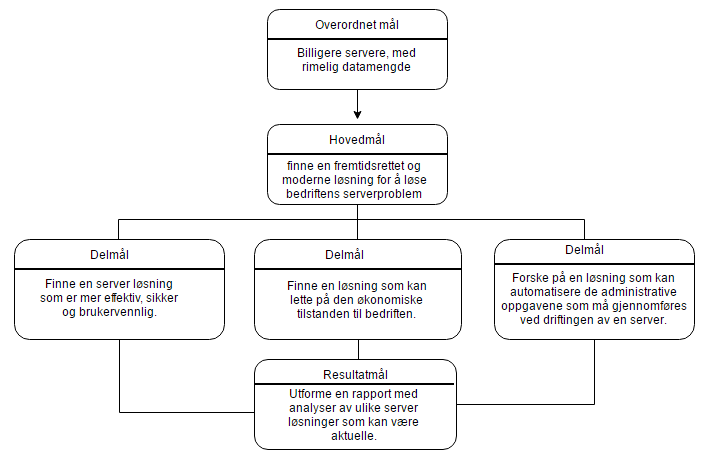
\includegraphics[width=6.5in]{Bilder/maal.PNG}
\caption{Prosjektets mål og resultatkrav}
\end{figure}

\section{Forutsetninger og rammer}

\paragraph{}Katoplast AS var åpne for at prosjektet og gruppen kunne ta fatt på oppgaven fra flere ulike vinkler, uten for mange avgrensninger og rammer som kunne eventuelt hindre sluttrapporten å oppnå beste kvalitet. Prosjekteierne ønsket ikke å begrense gruppen for mye og fokuserte hovedsakelig kun på noen små avgrensninger, som prosjektet måtte forholde seg til. Dette er svært positivt for gruppen ettersom det vil bli lettere å utforme analyser av ulike serverløsninger som kan være aktuelle for bedriften å velge. Flere muligheter vil bli dekket, og Katoplast vil kunne ha et større utvalg av løsninger når de til slutt skal velge den veien de ønsker å gå for. Katoplast var mest foukserte på sikkerhet, og var usikre når det gjaldt sky-løsninger. 

\section{Rapportstruktur}
\paragraph{} Prosjektet er delt opp i flere kapitler som tar for seg ulike områder for å skape en helhetlig rapport som er detaljert, men samtidig  enkel å forstå. Kapittel 1 av rapporten vår tar for seg introduksjonen av prosjektet. Her presenterer gruppen seg selv, oppdragsgiveren, hva oppdraget er og hva vi ønsker å oppnå og hvilke forutsetninger som er satt for prosjektet.

\paragraph{} Det neste kapittelet, kapittel 2, tar for seg teori og ulik fagstoff for prosjektet. Her beskrives vanskelig terminologi, og ulike konsepter som er viktig å forstå og vite hva er før en går videre med å lese prosjektet. Kapittel 2 er viktig for å skape et forståelig bilde av hele rapporten og de ulike analysene som er blitt gjort. Det vil finnes mange vanskelige begreper og uttrykk og teori kapittelet vil være til god hjelp for å forstå disse. I dette kapittelet beskrives de ulike delene ved servere og nettskyer, og de ulike tjenestene forklares.

\paragraph{} Det tredje kapittelet tar for seg metode. Altså hvilke metoder som ble benyttet for å finne frem til informasjon og hente ut informasjon. Den tar for seg de ulike metodene som gruppen benyttet, fra intervju til nettsøk til spørreundersøkelser. Den inkluderer også en situasjonsanalyse av bedriften for å få et bedre bilde av hvilken situasjon bedriften befinner seg i. Situasjonsanalysen er viktig for metode, ettersom den er viktig for innhentingen av informasjon for de senere analysene.

\paragraph{} Det fjerde kapittelet tar for seg de mange resultatene som gruppen har kommet til etter å ha gjennomført metodene, og med en situasjonsanalyse i bakhode. Her tar prosjektet for seg en arbeidskravsanalyse for å forstå hva som bør legges vekt på i analysene av de ulike løsningene, samt de mange resultatene som følge av forskningen som ble gjort på de ulike løsningene som gruppen har valgt å fokusere på. Her finner man resultatene av spørreundersøkelsen og et diagram som viser prisen på de ulike løsningene. 

\paragraph{} Kapittel 5 er diskusjonsdelen og diskuterer de ulike løsningene opp mot arbeidskravsanalysen og situasjonsanalysen som har blitt dannet. Diskusjons delen tar for seg de ulike løsningene for interne servere, sky tjenester og hybride løsninger som er viktige for Katoplast å vite. Dette er den viktigste delen av prosjektet ettersom den tar for seg hvordan de ulike løsningene kan påvirke Katoplast sin situasjon, og hvilken pris hver og en av de har.

\paragraph{} Avslutningsvis, så kommer konklusjonen som er det sjette og siste kapittelet. Konklusjonen tar for seg avslutningen på rapporten og vil komme med en anbefaling på hvilken løsning prosjektgruppen mener er den beste for bedriften Katoplast. Konklusjonen vil oppsummere hele prosjektet og prosjektgruppen vil ta et valg ut i fra den forskningen og de resultatene som gruppen har samlet sammen. 
\footnote{https://wiki.hiof.no/index.php/Bacheloroppgaven}
\chapter{Teori}
\paragraph{} Dette kapittelet vil gå dypere inn på den teoretiske delen rundt selve oppgaven. Her beskrives de grunnleggende elementene som benyttes i prosjektet, hva de betyr og hvordan de fungerer. I tillegg blir ulik terminologi som benyttes i rapporten forklart her og det er dermed nødvendig å lese og forstå denne delen før en fortsetter med å lese rapporten. Med dette ønsker gruppen å øke forståelsen til leseren og danne et bedre grunnlag for de som leser rapporten. Dette vil hjelpe med å velge den beste løsningen for bedriften.
\section{Grunnleggende elementer}
\paragraph{Hva er en server?} 
En server er et datamaskinprogram som forsørger forskjellige tjenester til forskjellige programmer og deres brukere. Datamaskinen serverprogrammet kjører på refereres til som en “server”. Servere deles ofte inn i forskjellige kategorier basert på hvordan de brukes, f.eks. en “Web Server” \footnote{http://whatis.techtarget.com/definition/server}

\paragraph{Hva er en nettsky?}  

En fremtidsrettet teknologi hvor data og informasjon lagres på servere som ligger på eksterne steder som er tilknyttet internett Nettskyen tillater brukere å lagre informasjon uten å behøve å selv drifte en egen server. Microsoft, Google, og Amazon. Nettskybasert databehandling tilbyr en rekke fordeler for fortetninger og brukere. Vi kan dele fordelene inn i 3 forskjellige grupperinger.\footnote{https://no.wikipedia.org/wiki/Nettskyen}.

\paragraph{Hva er en hybridløsning?} 

En hybrid-løsning i prosjektet handler om å finne en mulig vei for bedriften med blandede løsninger som kan være aktuelt å bruke. For eksempel, å bruke både interne servere som blir plassert hos bedriften og en liten cloud-løsning som befinner seg hos en annen leverandør.
Dette er noe som kan være aktuelt hvis bedriften ønsker å ha noe av dataene sine på huset.\footnote{http://www.dummies.com/programming/cloud-computing/hybrid-cloud/what-is-hybrid-cloud-computing/}

\paragraph{} Nettskyen, skyen eller cloud er en fellesbetegnelse på alt fra dataprosessering og datalagring til programvare på eksterne servere tilknyttet Internett. (En server er en programvare som tilbyr en eller flere tjenester over et datanettverk. Begrepet server, eller tjener på norsk er også ofte brukt på maskinvaren som programmet/programmene kjøres fra, så lenge maskinen har kapasiteten til å utføre oppgavene.

Vi kan også dele skytjenestene opp i forskjellige leveransemodeller. Da går det altså hovedsakelig ut på allmenn tilgjengelig {\small (Public Cloud)}, privat tilgjengelig {\small (Private Cloud)} og sist hybridsky {\small (Hybrid Cloud)};\par
\begin{description}[noitemsep]
\item[Public Cloud] En allmenn tilgjengelig sky betyr at skytjeneste er gjort tilgjengelig for alle kunder av leverandøren.
\item[Private Cloud] Privat tilgjengelig sky betyr at skytjenesten er gjort privat, og dedikert kun til en gruppe av kunder. Skytjenesten gjelder altså kun for virksomheten den er dedikert til. Som vi ser, her vil skyen typisk bli dedikert til den enkelte kunden eller den definerte kundegruppen. Denne løsningen åpner for en større grad av spesifikke tilpasninger.
\item[Hybrid Cloud] Hybrid sky er altså en blanding av tjenestene som kan leveres ovenfor. En god blanding av de begge.
\end{description}
\begin{figure}[H]
\centering
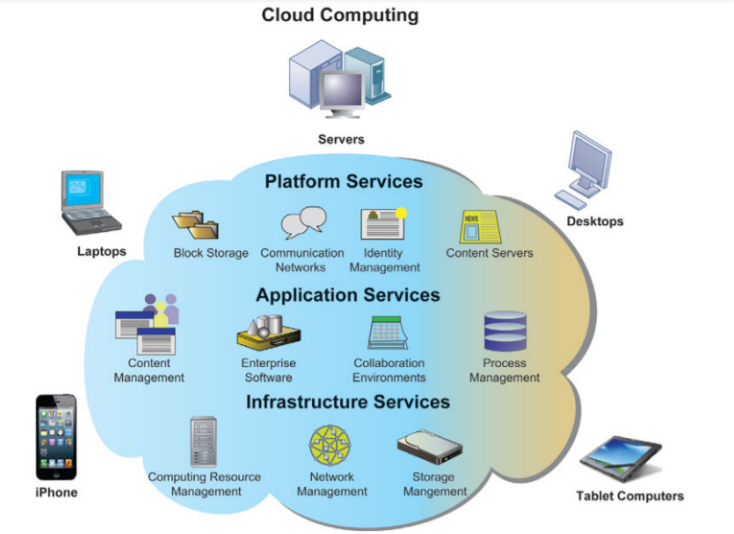
\includegraphics[width=6.5in]{Bilder/cc.PNG}
\caption{En visuell representasjon av hvordan Sky tjenester er satt opp.(Laudon \& Laudon, 2016, s.223)}
\end{figure}

Som vi kan lese ovenfor, tilbyr skybaserte løsninger en rekke forskjellige modeller. Disse modellene er veldig fleksible, brukervennlige og tilpasset behov. Under vil du finne ulike skytjenester som tilbys fra bedrifter som Microsoft, Amazon og Google:
\begin{description}
\item Microsoft Azure er en skytjeneste som er utviklet av Microsoft og som tilbyr brukere av tjenesten en rekke verktøy og programmer knyttet til lagring, utvikling og distribuering av informasjon og data.\footnote{https://azure.microsoft.com/nb-no/}

\item Amazon Web Services (AWS) er Amazon sitt svar på en skytjeneste. Med Amazon AWS har man tilgang til en rekke funksjoner, deriblant muligheten til å enkelt lagre store og små datamengder, levere ulikt innhold til brukere og kraftige maskiner som tar seg av mye av arbeidet.\footnote{https://aws.amazon.com/about-aws/}

\item Google Disk er en versjon av en Sky tjeneste forenklet så mye som mulig for å tilpasse så mange brukere som mulig. Med Google Disk har man tilgang til alle filene og mappene sine, uansett hvor man er, med et svært enkelt brukergrensesnitt og hvor mye av de administrative oppgavene blir tatt hånd om.\footnote{https://www.google.com/drive/}

\item Microsoft PowerShell er et komandolinjeskall for systemadministratorer. PowerShell fungerer i form av at systemadministrator skriver inn kommando for å styre operativsystemet til å utføre bestemte oppgaver. Det å arbeide i PowerShell kan få brukeren til å styre programmer og manipulerer elementer i systemets database. Når det er nevnt kreves det noe datakunnskaper for å utføre disse manipulasjonene. \footnote{http://www.datamaskin.biz/Systems/windows/212342.html}
\end{description}

\section{Server}
\paragraph{} En server er et datamaskinprogram som forsørger forskjellige tjenester til forskjellige programmer og deres brukere. Datamaskinen serverprogrammet kjører på refereres til som en “server”. Servere deles ofte inn i forskjellige kategorier basert på hvordan de brukes, f.eks. en “Web Server” \todo[author=Ole]{{\scriptsize Bruk heller enquotes}} 
\begin{figure}[H]
\centering
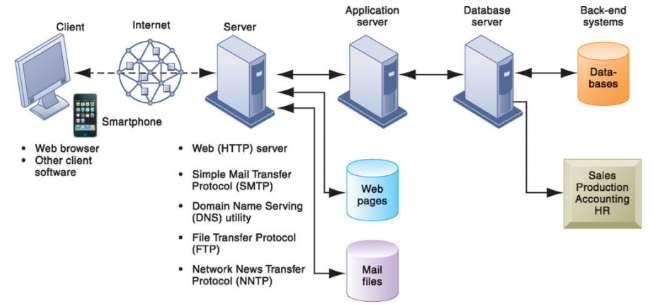
\includegraphics[width=6.5in]{Bilder/cc2.PNG}
\caption{En modell som viser en visuell forklaring på hvordan datamaskiner, Internet og servere henger sammen med andre systemer. (Laudon \& Laudon, 2016, s.305) }
%\todo[inline,author=Ole]{{\scriptsize Dere må ref'e til hvor dette bildet er tatt fra. Ved å linke til bibliografien deres. Dette må dere gjøre med ALLE bilder og grafikk dere har hentet fra andre kilder en dere selv. Dette gjør dere ved å bruke \textbackslash cite\{labeltype:refname\}}}
\end{figure}

\section{Terminologi}
\paragraph{} {\bfseries Interne servere:} Interne servere i en bedrift vil si at serveren står fysisk i lokalene til selskapet. Disse serveren vil altså lagre data, kjøre applikasjoner og holde på forskjellige API/ERP løsninger som selskapet benytter. \footnote{https://no.wikipedia.org/wiki/Server}
\footnote{http://whatis.techtarget.com/definition/server}

\paragraph{} {\bfseries ERP:} Enterprise resource planning (ERP) er en programvare som støtter flere av en bedrifts virksomgetsområder,  som produksjon, lager, salg , innkjøp og økonomi.  Målet med ERP er å håndtere virksomgetens informasjon.
\footnote{https://www.oracle.com/applications/erp/what-is-erp.html}

\paragraph{} {\bfseries Operativsystem:} Et operativsystem (OS) er den grunnleggende programvaren på en datamaskin, og det som tildeler de forskjellige ressursene i datamaskinen til andre programmer.
\footnote{https://no.wikipedia.org/wiki/Operativsystem}

\paragraph{} {\bfseries PaaS(Platform as a service):}  Plattform som en tjeneste eller applikasjonsplattform som en tjeneste (aPaaS) er en kategori av cloud 
computing-tjenester som gir en plattform som gjør det mulig for kunder å utvikle, kjøre og administrere applikasjoner 
uten kompleksiteten i å bygge og vedlikeholde infrastrukturen som vanligvis er knyttet til å utvikle Og lanserer en app.
\footnote{https://en.wikipedia.org/wiki/Platform\_as\_a\_service}

\paragraph{} {\bfseries IaaS(Infrastructure as a Service):} Infrastruktur som en tjeneste er en form for cloud computing som gir databehandlings ressurser over Internett.
\footnote{http://searchcloudcomputing.techtarget.com/definition/Infrastructure-as-a-Service-IaaS}

\paragraph{} {\bfseries SaaS(Software as a Service):} Programvare som en tjeneste er en programvaredistribusjonsmodell 
der en tredjepartsleverandør er vert for programmer og gjør dem tilgjengelige for kunder over Internett.
\footnote{http://searchcloudcomputing.techtarget.com/definition/Software-as-a-Service}

\paragraph{} {\bfseries Data:} Informasjon, brukes for grunnlag av begrynnelse, diskusjon eller beregninger. 
\footnote{https://www.merriam-webster.com/dictionary/data}

\paragraph{} {\bfseries API:} Application Programming Interface, er et programfunksjon som lar brukeren koble sammen flere programmer.  Man kan da utveksle informasjon på tvers av programmene. 
\footnote{}
\paragraph{} {\bfseries Programvare:} Programvare (engelsk: software) er en fellesbetegnelse på dataprogrammer. Alt som er digitalt i dag har en form for programvare. 
\footnote{http://www.computerhope.com/jargon/s/software.htm}

\paragraph{} {\bfseries Maskinvare:} Maskinvare er de fysiske delene en server/datamaskin består av.
\footnote{http://www.computerhope.com/jargon/h/hardware.htm}
\footnote{http://www.computerhope.com/issues/ch000039.htm}

\paragraph{} {\bfseries Skytjenste (Cloud):} En Skytjeneste (Cloud) er et sett med applikasjoner, tjenester, lagring og maskinvare som opprettholdes og driftes av en tredje-part, som tillater andre bedrifter og organisasjoner å enkelt kunne lagre data og informasjon, uten å måtte bry seg om det tunge, administrative arbeidet som må gjøres for å drifte en slik løsning. Skytjenestene tillater brukere å lagre informasjon og data på en server som befinner seg på et eksternt sted på internett for å gjøre det så enkelt som mulig for brukeren.
\footnote{https://www.datatilsynet.no/Teknologi/Skytjenester---Cloud-Computing/Hva-er-nettskytjenester/}
\footnote{https://www.anskaffelser.no/it/temaer-it/skytjenester-cloud}

\paragraph{} {\bfseries Hybrid Cloud:} En "Hybrid Cloud" eller en hybrid skytjeneste, er en form for Skytjeneste som kombinerer og blander tjenestene og egenskapene fra de grunnleggende formene for nettskyer, Public og Private cloud og tilbyr brukerne å benytte seg av en blanding av disse for å oppnå et enhetlig, sikkert og automatisert lagrings system for både viktig og mindre viktig data og informasjon innenfor bedriften.
\footnote{https://www.microsoft.com/nb-no/cloud-platform/hybrid-cloud}

\paragraph{} {\bfseries SSD:} Solid State Drive (SSD) er en nyere form for harddisk (maskinvare) som benyttes som et lagringsmedium hvor søketiden og lagringen foregår med høyere hastighet enn med en vanlig harddisk. Som følge av den kjappere lagringen som en SSD kan gjennomføre, koster også disse harddiskene mer enn de vanlige harddiskene.
\footnote{https://www.komplett.no/category/10088/datautstyr/lagring/harddisker/ssd}
\footnote{http://uk.pcmag.com/storage-devices-reviews/8061/feature/ssd-vs-hdd-whats-the-difference}

\paragraph{} {\bfseries HDD:} Hard Disk Drive (HDD) er den tradisjonelle formen for en harddisk og er et lagringsmedium som er tilstrekkelig brukt i verden. Slike tradisjonelle harddisker har ofte en rekke ulemper ved seg, blant annet at de er sårbare og ikke minst tregere med å gjennomføre lagring enn nyere harddisker.
\footnote{http://uk.pcmag.com/storage-devices-reviews/8061/feature/ssd-vs-hdd-whats-the-difference}


\paragraph{} {\bfseries iSCSI:} Internet Small Computer Systems Interface (iSCSI) er en internet protokoll som står for den lagringen som gjennomføres over internett. iSCSI håndterer lagringen av data over internett, hvor det ikke er noen begrensning på avstander. Store organisasjoner benytter seg av denne protokollen hvor de tar imot informasjon og data fra andre brukere og lagrer disse i store datasentre. Kundene kan dermed gjennomføre lagring uten behov for fysiske harddisker.
\footnote{https://no.wikipedia.org/wiki/ISCSI}

\paragraph{} {\bfseries DDOS-angrep:} Et DDOS-angrep (distribuert tjenestenekt) er en form for Internett angrep hvor maskinene til et offer angripes og hvor brukeren, som blir angrepet, hindres i å gjennomføre handlinger eller få tilgang til informasjon. Dette kjennetegnes ofte ved man mister Internet tilgang. Dette kan føre til stor nedetid og koste dyrt for de som angripes.
\footnote{http://www.digitalattackmap.com/understanding-ddos/}
\footnote{https://no.wikipedia.org/wiki/Tjenestenektangrep}

\paragraph{} {\bfseries Ulovlig Hacking:} Ulovlig Hacking er en form for datakriminalitet hvor en person benytter sine ferdigheter, programmer og løsninger for å bryte seg inn og ulovlig hente informasjon eller manipulere data hos andre personer eller bedrifter. Dette kan føre til store konsekvenser for de som blir utsatt hvor sensitive opplysninger kan bli lekket. 
\footnote{https://snl.no/hacker}

\paragraph{} {\bfseries Nano Server:} Nano Server er et helt nytt og fremtidig konsept som er utviklet av Microsoft og som gir deg muligheten til å fjernstyre operativsystemene til en windows server og som er optimalisert for skytjenester. Fordelen med dette er at den tar opp svært lite plass, er merkbart raskere og behøver mindre oppdateringer enn de tradisjonelle serverne.
\footnote{https://www.pluralsight.com/blog/it-ops/microsoft-nano-server-announced}
\footnote{https://technet.microsoft.com/en-us/windows-server-docs/get-started/getting-started-with-nano-server}

\paragraph{} {\bfseries OpenStack:} OpenStack er programvare som benyttes av leverandører av nettskyer hvor alle ressursene knyttet til programvaren er frie og åpne til allmennheten slik at de kan benyttes og endres på akkurat slik man ønsker. Dette tillater for nye ideer og metoder for nettskyer.
\footnote{https://www.openstack.org/}

\paragraph{} {\bfseries OpenSource:} Programvare som har OpenSource-lisens er programvare som tillater andre personer å endre, manipulere og distribuere programvaren akkurat som de ønsker uten at dette skal få noen konsekvenser. Dette åpner for store muligheter for både brukere og utviklere.
\footnote{https://opensource.com/resources/what-open-source}

\paragraph{} {\bfseries Virtuell maskiner:} En virtuell maskin er en programvare-simulering av en komplett datamaskin som utfører programmer på samme måte som en fysisk datamaskin. Med en slik fysisk maskin kan man kjøre simulering av flere maskiner, også med ulike operativsystemer. Hvis en benytter Windows 7 som hovedoperativsystem, men er avhengig av en virtuell maskin med Windows 10 på grunn av et program man er avhengig av i jobbsammenheng- kan man bare bytte om på operativsystemet sitt ved hjelp av en slik maskin. \footnote{https://it.uib.no/Virtuell\_maskin}

\include{conclusions}

%now enable appendix numbering format and include any appendices
\appendix
\include{appendix1}
\include{appendix2}

%next line adds the Bibliography to the contents page
\addcontentsline{toc}{chapter}{Bibliography}
%uncomment next line to change bibliography name to references
%\renewcommand{\bibname}{References}
\bibliography{refs}        %use a bibtex bibliography file refs.bib
\bibliographystyle{plain}  %use the plain bibliography style

\end{document}
